\documentclass{beamer}
\usepackage{config}

%Information to be included in the title page:
\title[Git collaboratif]{Git à plusieurs : mode d'emploi}
\author{Florian Legendre}
\institute{Université de Poitiers}
\date{Année 2020 - 2021}
\logo{
\includegraphics[scale=0.1]{UP.png}}


%%% ============================================================= %%%
%%% ====================== Début des diapos ===================== %%%
%%% ============================================================= %%%

\begin{document}

\frame{\titlepage}

\begin{frame}
\frametitle{Table of Contents}
\tableofcontents[hideallsubsections]
\end{frame}


%% --------------------- %%
%%        SECTION        %%
%% --------------------- %%
\AtBeginSection[]
{
  \begin{frame}
    \frametitle{Table of Contents}
    \tableofcontents[sectionstyle=show/hide,subsectionstyle=show/show/hide]
  \end{frame}
}

\section{Les interdictions de push}

% Subsection:
\subsection{Quelques remarques préliminaires}
\begin{frame}{Git n'est pas GitHub!}

À l'instar des branches où je considérais que vous aviez un dépôt distant et où je vous  montrais comment configurer vos branches locales/distantes depuis Git, ici je vais vous présenter deux dernières notions de Git qui sont indépendantes du choix de dépôt distant que vous ferez.\\
\medskip

Ces notions sont celles d'interdictions de push et de conflits d'édition. Bien que le mot "conflit" puisse faire peur il s'agit de quelque-chose de tout à fait ordinaire quand on travaille à plusieurs sur un même projet. Git simplifie grandement la gestion de ces conflits.\\

\end{frame}




%% --------------------- %%
%%        SECTION        %%
%% --------------------- %%
\AtBeginSection[]
{
  \begin{frame}
    \frametitle{Table of Contents}
    \tableofcontents[sectionstyle=show/hide,subsectionstyle=show/show/hide]
  \end{frame}
}

\section{Rappels sur les conflits d'édition}

% Subsection:
\subsection{Rappel de la notion de conflits d'édition}
\begin{frame}{Rappel du problème}
\begin{center}
    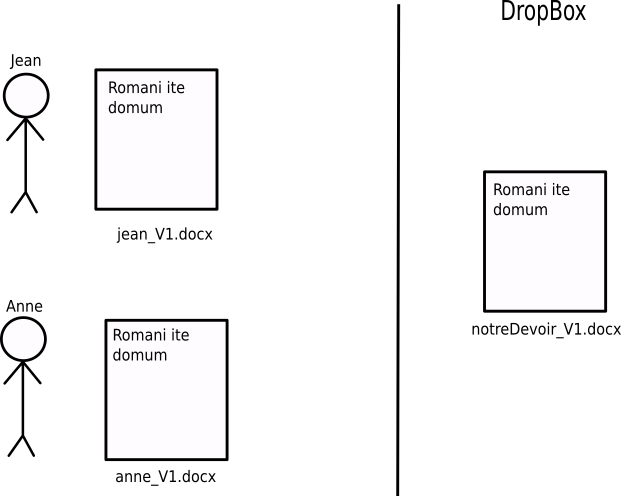
\includegraphics[scale=0.4]{lastScenario/lastScenario_init.png}
\end{center}
\end{frame}

\begin{frame}{Rappel du problème}
\begin{center}
    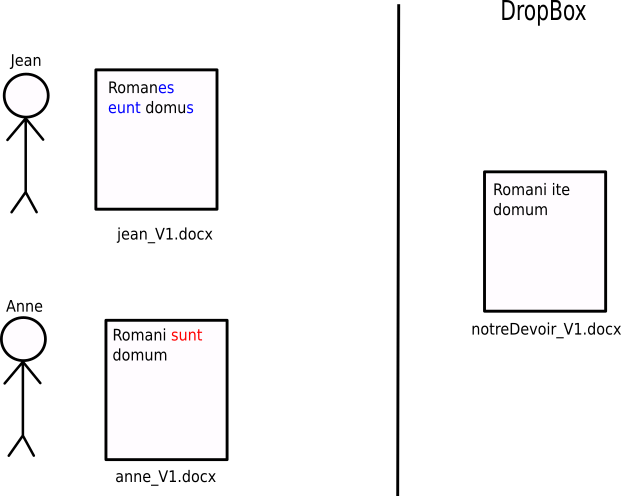
\includegraphics[scale=0.4]{lastScenario/lastScenario_conflict1.png}
\end{center}
\end{frame}

\begin{frame}{Rappel du problème}
\begin{center}
    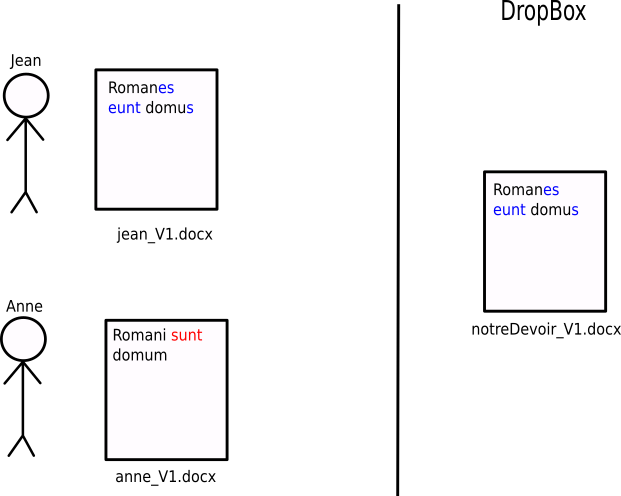
\includegraphics[scale=0.4]{lastScenario/lastScenario_conflict2.png}
\end{center}
\end{frame}

\begin{frame}{Rappel du problème}
\begin{center}
    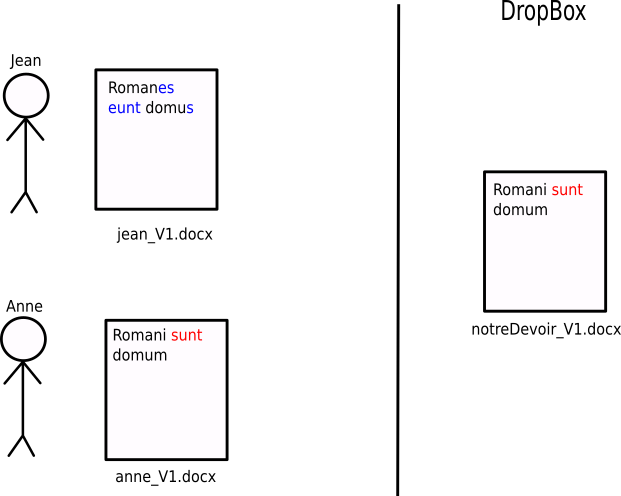
\includegraphics[scale=0.4]{lastScenario/lastScenario_conflict3.png}
\end{center}
\end{frame}

\begin{frame}{Rappel de la solution "à la main"}
\begin{center}
    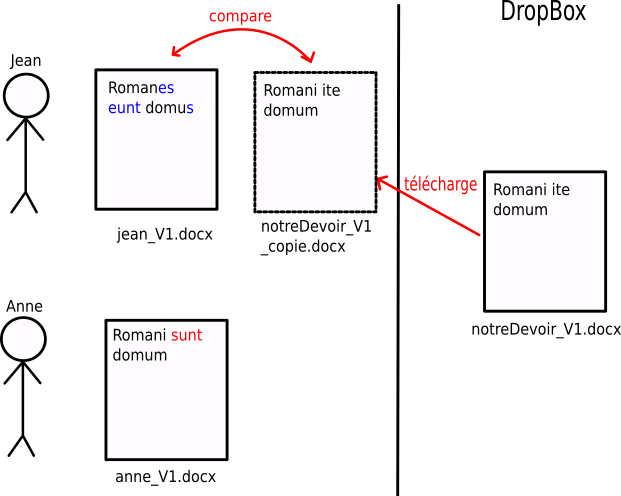
\includegraphics[scale=0.4]{lastScenario/lastScenario_pullpush1.png}
\end{center}
\end{frame}

\begin{frame}{Rappel de la solution "à la main"}
\begin{center}
    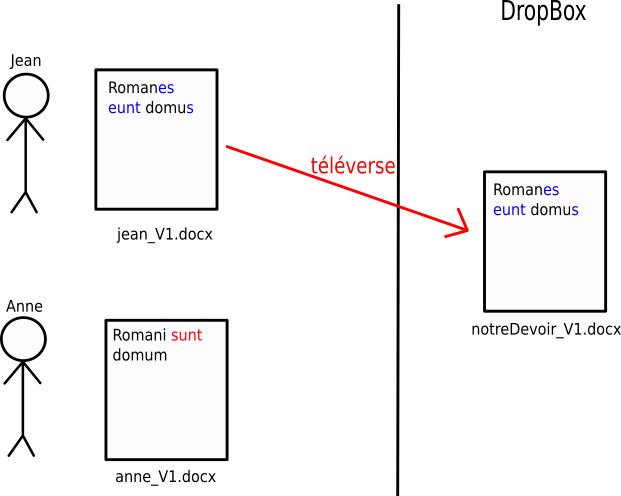
\includegraphics[scale=0.4]{lastScenario/lastScenario_pullpush2.png}
\end{center}
\end{frame}

\begin{frame}{Rappel de la solution "à la main"}
\begin{center}
    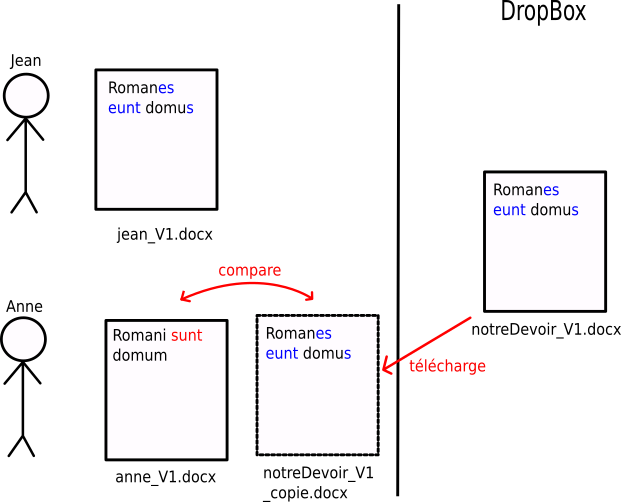
\includegraphics[scale=0.4]{lastScenario/lastScenario_pullpush3.png}
\end{center}
\end{frame}


% Subsection:
\subsection{Quel est le rôle de Git dans la gestion de ces conflits?}
\begin{frame}{Rôle de Git}

Git ne peut pas décider à votre place de ce qui doit être supprimé ou gardé! Ou alors nous perdons tous notre travail car les ordinateurs peuvent coder...\\
\medskip

Mais Git peut vous indiquer dans quels fichiers et à quelles lignes vos deux versions sont en conflit. 
    
\end{frame}


%% --------------------- %%
%%        SECTION        %%
%% --------------------- %%
\AtBeginSection[]
{
  \begin{frame}
    \frametitle{Table of Contents}
    \tableofcontents[sectionstyle=show/hide,subsectionstyle=show/show/hide]
  \end{frame}
}

\section{Gestion des conflits d'édition avec Git}


% Subsection:
\subsection{Git fait la détection}

\begin{frame}[fragile]{Un conflit détecté par Git}
Un conflit survient quand on met à jour sa branche locale avec la branche distante suivie et qu'une ou plusieurs versions de la branche suivie fait état de zones éditées qui sont en conflit avec celles de notre branche locale:
\begin{mdframed}[style=Bash]
\begin{lstlisting}[style=Bash, caption={Exemple de détection automatique de conflit d'édition}]
crex@crex:~/projects/GitLearn(dev)$ git pull
remote: Enumerating objects: 7, done.
remote: Counting objects: 100% (7/7), done.
remote: Compressing objects: 100% (2/2), done.
remote: Total 4 (delta 1), reused 0 (delta 0), pack-reused 0
Unpacking objects: 100% (4/4), 705 bytes | 16.00 KiB/s, done.
From github.com:Chuxclub/GitLearn
   a223800..d261500  dev        -> origin/dev
Auto-merging codes/test.txt
CONFLICT (content): Merge conflict in codes/test.txt
Automatic merge failed; fix conflicts and then commit the result.
\end{lstlisting}
\end{mdframed}
\end{frame}

\begin{frame}[fragile]{Un conflit détecté par Git}

Pour savoir quels fichiers sont en conflits vous pouvez aussi utiliser la commande \textit{git status} qui vous renseigne en plus sur la marche à suivre:
\begin{mdframed}[style=Bash]
\begin{lstlisting}[style=Bash, caption=Les fichiers en conflit indiqués par git status]
crex@crex:~/projects/GitLearn(dev)$ git status
On branch dev
Your branch and 'origin/dev' have diverged,
and have 2 and 1 different commits each, respectively.
  (use "git pull" to merge the remote branch into yours)

You have unmerged paths.
  (fix conflicts and run "git commit")
  (use "git merge --abort" to abort the merge)

Unmerged paths:
  (use "git add <file>..." to mark resolution)
	both modified:   codes/test.txt

no changes added to commit (use "git add" and/or "git commit -a")
\end{lstlisting}
\end{mdframed}
\end{frame}

\begin{frame}{Un conflit détecté par Git}
Normalement à chaque fois que vous mettez à jour votre branche locale en faisant un \textit{git pull}, git crée un commit qui enregistre cette mise à jour (comme ça il est facile de défaire une mise à jour avec un \textit{git revert <id>}).\\
\medskip

Cependant, quand Git détecte un conflit il attend que vous ayiez résolu ce-dernier avant de faire un commit de la mise à jour.
\end{frame}

\begin{frame}[fragile]{Un conflit détecté par Git}
Lors d'un conflit Git \textbf{\underline{écrit dans}} le fichier conflictuel comme ci-dessous:
\smallskip
\begin{center}
	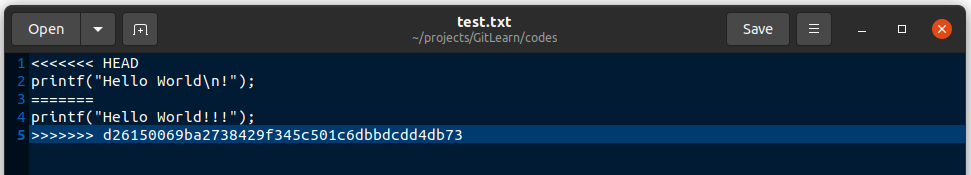
\includegraphics[scale=0.3]{gestionConflits1.png}
\end{center}
\end{frame}

\begin{frame}[fragile]{Un conflit détecté par Git}
Vous remarquerez les deux parties crées par les $<<<$, $===$ et $>>>$ de Git. La première partie (HEAD) correspond à ce qu'il y a chez vous (Rappel: HEAD = "vous êtes ici pour Git"), la seconde partie correspond à ce qu'il y a sur la branche distante:
\smallskip
\begin{center}
	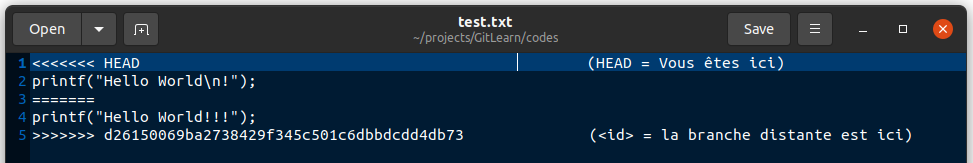
\includegraphics[scale=0.3]{gestionConflits2.png}
\end{center}
\end{frame}


% Subsection:
\subsection{Vous faites la résolution}
\begin{frame}{Vous faites la résolution}
Git vous a épargné la détection des conflits. Mais la gestion/résolution reste à votre charge! Pour ce faire il suffit d'aller dans le fichier conflictuelle/édité par Git et de supprimer/garder les lignes qui vous intéressent.
\end{frame}

\begin{frame}{Vous faites la résolution}
Je peux faire ce que je veux lors d'une édition de conflits: garder tout ou partie ou rien du tout du travail de mon collègue ou le mien. Vous faites ce choix selon vos besoins. Ici je choisis de supprimer entièrement le travail qui était sur la branche distante:\\
\smallskip

\begin{center}
	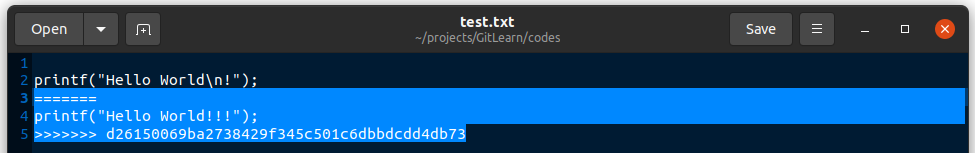
\includegraphics[scale=0.3]{gestionConflits3.png}\\
	\vspace{0.5cm}
	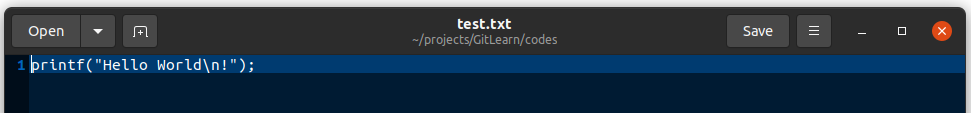
\includegraphics[scale=0.3]{gestionConflits4.png}
\end{center}
\end{frame}

\begin{frame}[fragile]{Vous faites la résolution}
Une fois que vous avez fini de choisir ce que vous vouliez garder ou non (discutez-en avec la personne concernée avant!) vous pouvez ajouter les fichiers au staging avec \textit{git add <nom\_fichier>} afin de préparer le commit que Git a suspendu en vous attendant:

\begin{mdframed}[style=Bash]
\begin{lstlisting}[style=Bash, caption=Fin de résolution du conflit]
crex@crex:~/projects/GitLearn(dev)$ git add -A
crex@crex:~/projects/GitLearn(dev)$ git status
On branch dev
Your branch and 'origin/dev' have diverged,
and have 2 and 1 different commits each, respectively.
  (use "git pull" to merge the remote branch into yours)

All conflicts fixed but you are still merging.
  (use "git commit" to conclude merge)

Changes to be committed:
	modified:   codes/test.txt
crex@crex:~/projects/GitLearn(dev)$ git commit -am "Conflit résolu"
[dev 313203f] Conflit résolu
\end{lstlisting}
\end{mdframed}
\end{frame}


\end{document}